\section{Results}
\label{sec:results}

\subsection{Detection performance}
\label{sec:res-main}
Table~\ref{tab:main} gives cluster-aware, out-of-fold AUROC for the logistic regression, the PSSM, and their consensus (Eq.~\ref{eq:cons}). Discrimination is well above chance for every protease, ranging from \aucConsMMPnine{} for MMP-9 to \aucConsFaecal{} for the faecal group. The serine-protease models (NE, faecal) and LasB are best, the MMPs least so. The consensus is at or near the best single scorer for all proteases; for MMP-2 and MMP-8 the PSSM alone is slightly higher, with overlapping intervals. Secondary metrics are in Table~\ref{tab:secondary}; Figure~\ref{fig:roc} shows ROC and precision-recall curves.

\begin{table}[!htbp]
\centering\small{\footnotesize\begin{tabular}{@{}lrrccc@{}}\toprule
Protease & Positives & Positive clusters & LR AUROC & PSSM AUROC & Consensus AUROC \\\midrule
MMP-2 & 2,819 & 2,608 & 0.854 \,[0.844, 0.863] & \textbf{0.874 \,[0.863, 0.883]} & 0.869 \,[0.859, 0.878] \\
MMP-8 & 698 & 677 & 0.755 \,[0.733, 0.774] & \textbf{0.784 \,[0.762, 0.800]} & 0.783 \,[0.763, 0.800] \\
MMP-9 & 783 & 687 & 0.760 \,[0.723, 0.791] & 0.761 \,[0.723, 0.798] & \textbf{0.772 \,[0.737, 0.803]} \\
MMP-14 & 717 & 705 & 0.772 \,[0.753, 0.790] & 0.785 \,[0.766, 0.806] & \textbf{0.791 \,[0.771, 0.810]} \\
Neutrophil elastase & 327 & 324 & 0.895 \,[0.875, 0.913] & 0.885 \,[0.861, 0.906] & \textbf{0.901 \,[0.880, 0.919]} \\
LasB & 128 & 106 & 0.877 \,[0.835, 0.917] & 0.881 \,[0.837, 0.916] & \textbf{0.887 \,[0.844, 0.923]} \\
Faecal serine proteases & 5,000 & 4,715 & 0.951 \,[0.948, 0.954] & 0.953 \,[0.950, 0.956] & \textbf{0.953 \,[0.950, 0.956]} \\
\bottomrule\end{tabular}}

\caption{Cluster-aware $5$-fold cross-validated AUROC with $95\%$ cluster-bootstrap intervals (bold: highest of the three scorers). ``Positive clusters'' is the number of distinct near-duplicate clusters among the positives.}
\label{tab:main}
\end{table}

\begin{table}[!htbp]
\centering\small\begin{tabular}{@{}lccccl@{}}\toprule
Protease & PR-AUC & MCC & Brier & ECE & $C$ chosen per outer fold \\\midrule
MMP-2 & 0.649 & 0.521 & 0.156 & 0.153 & 0.1, 0.1, 0.1, 0.1, 0.1 \\
MMP-8 & 0.474 & 0.346 & 0.202 & 0.199 & 0.01, 0.01, 0.01, 0.01, 0.01 \\
MMP-9 & 0.535 & 0.335 & 0.196 & 0.196 & 0.01, 0.01, 0.01, 0.01, 0.01 \\
MMP-14 & 0.516 & 0.370 & 0.195 & 0.191 & 0.1, 0.01, 0.01, 0.1, 0.01 \\
Neutrophil elastase & 0.751 & 0.600 & 0.127 & 0.114 & 0.1, 0.1, 0.1, 0.1, 0.1 \\
LasB & 0.783 & 0.602 & 0.125 & 0.122 & 0.01, 0.1, 0.1, 0.1, 0.01 \\
Faecal serine proteases & 0.800 & 0.806 & 0.071 & 0.055 & 1.0, 0.1, 1.0, 0.1, 0.1 \\
\bottomrule\end{tabular}

\caption{Secondary metrics for the logistic regression. PR-AUC is measured against a prior of $0.25$; MCC at threshold $0.5$; ECE under the training prior. Selected $C$ is listed per outer fold.}
\label{tab:secondary}
\end{table}

\begin{figure}[!htbp]
\centering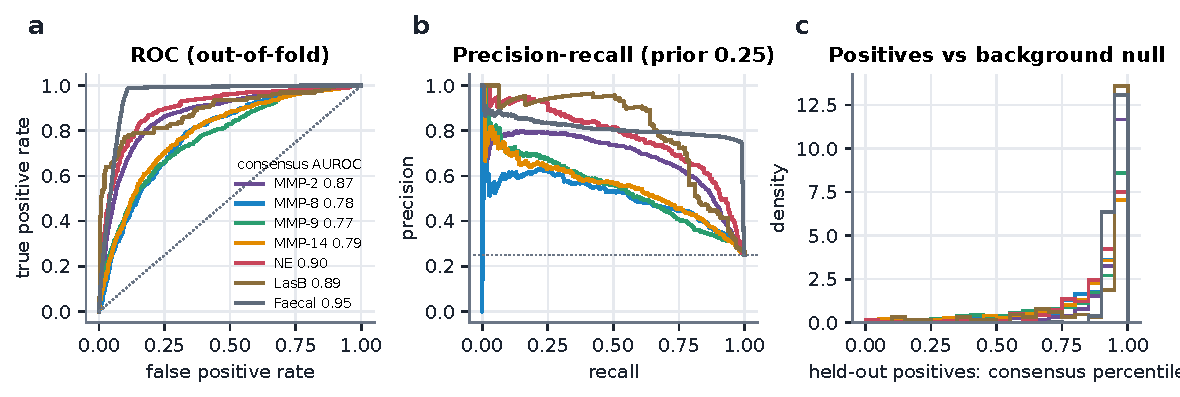
\includegraphics[width=\textwidth]{figures/F09_roc_pr.pdf}
\caption{Out-of-fold performance of the consensus score. \textbf{(a)} ROC curves. \textbf{(b)} Precision-recall curves. \textbf{(c)} Distribution of the consensus percentile of held-out positives; positives concentrate near the top of the background distribution for every protease.}
\label{fig:roc}
\end{figure}

\subsection{Which model, and which representation?}
\label{sec:res-models}
Figure~\ref{fig:models} and Table~\ref{tab:models} compare seven models on identical folds: a constant prior, a composition-only logistic regression, one-hot and VHSE logistic regressions, the PSSM, and gradient-boosted trees on both encodings. Three conclusions follow.

\begin{enumerate}
\item \textbf{Position matters; composition mostly does not.} For six of seven proteases, composition alone gives $0.60$--$0.74$ AUROC and the VHSE model beats it significantly (Table~\ref{tab:paired}); label-shuffled controls sit at chance (Table~\ref{tab:controls}). \textbf{LasB is the exception:} composition alone reaches $0.886$, statistically indistinguishable from the full model ($-0.008$, interval including zero). The LasB model is largely detecting elastin-like composition, as expected from a positive set that is $76\%$ elastin (Section~\ref{sec:limits}).
\item \textbf{There is no evidence of strong position--position interaction.} Gradient-boosted trees, which can represent interactions, reach within $0.013$ AUROC of the better of the one-hot regression and the PSSM on every protease and exceed it only on NE, by $0.007$. An additive model is adequate at these data sizes, and it is also the interpretable one.
\item \textbf{The representation trade-off is real.} On data-rich proteases (MMP-2, MMP-8) the one-hot logistic regression and the PSSM are significantly better than the VHSE model by $0.017$ to $0.034$ AUROC, consistent with the bias measured in Table~\ref{tab:controls}. On NE and LasB the VHSE model is significantly better than the one-hot model ($+0.021$ and $+0.033$). The learning curves (Figure~\ref{fig:lc}) show the same crossover: VHSE is ahead at small training sizes and is overtaken as data grow.
\end{enumerate}
The PSSM has no fitted hyperparameter and is at or within its interval of the best model everywhere, which is why the shipped score combines it with the logistic regression rather than choosing one.

\begin{figure}[!htbp]
\centering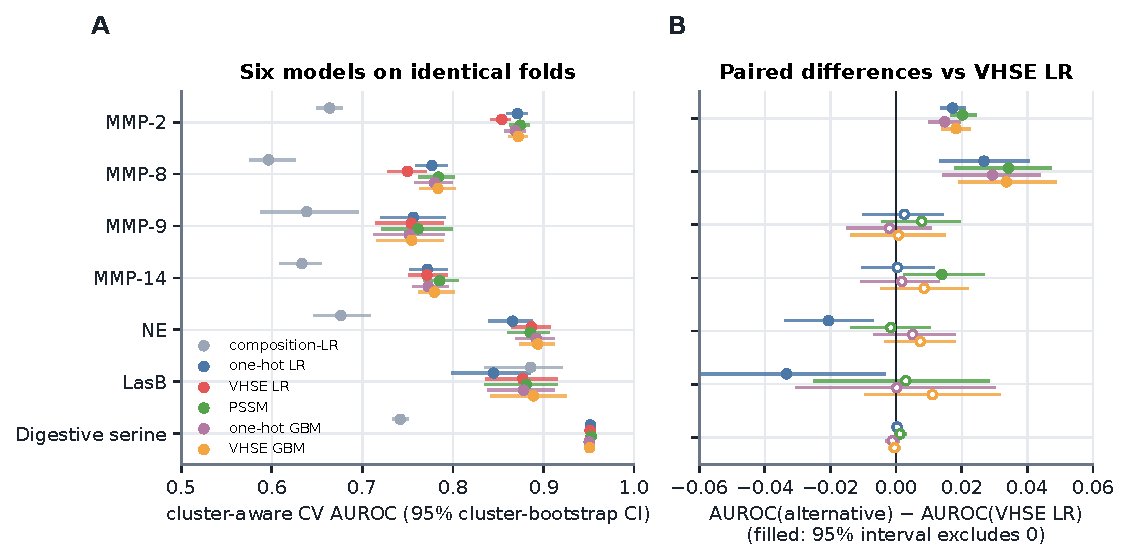
\includegraphics[width=\textwidth]{figures/F05_model_comparison.pdf}
\caption{\textbf{(a)} Cluster-aware AUROC of six models on identical folds with $95\%$ cluster-bootstrap intervals. \textbf{(b)} Paired difference (alternative minus VHSE LR); filled markers have intervals excluding zero. The composition-only model is $0.12$--$0.21$ AUROC below for every protease except LasB and is omitted from panel (b) for scale.}
\label{fig:models}
\end{figure}

\begin{table}[!htbp]
\centering\small\begin{tabular}{@{}lccccccc@{}}\toprule
Protease & Prior & Composition & One-hot LR & VHSE LR & PSSM & One-hot GBM & VHSE GBM \\\midrule
MMP-2 & 0.500 & 0.664 & 0.871 & 0.854 & \textbf{0.874} & 0.869 & 0.872 \\
MMP-8 & 0.500 & 0.596 & 0.777 & 0.750 & \textbf{0.784} & 0.780 & 0.783 \\
MMP-9 & 0.500 & 0.639 & 0.756 & 0.754 & \textbf{0.761} & 0.752 & 0.755 \\
MMP-14 & 0.500 & 0.633 & 0.772 & 0.771 & \textbf{0.785} & 0.773 & 0.779 \\
Neutrophil elastase & 0.500 & 0.676 & 0.866 & 0.887 & 0.885 & 0.892 & \textbf{0.894} \\
LasB & 0.500 & 0.886 & 0.845 & 0.877 & 0.881 & 0.878 & \textbf{0.889} \\
Faecal serine proteases & 0.500 & 0.742 & 0.952 & 0.951 & \textbf{0.953} & 0.950 & 0.951 \\
\bottomrule\end{tabular}

\caption{Cross-validated AUROC by model and protease (bold: best). The prior is constant and gives $0.5$.}
\label{tab:models}
\end{table}

\begin{table}[!htbp]
\centering\small\begin{tabular}{@{}lcccc@{}}\toprule
Protease & One-hot LR & PSSM & One-hot GBM & VHSE GBM \\\midrule
MMP-2 & +0.017$^{*}$ & +0.020$^{*}$ & +0.015$^{*}$ & +0.018$^{*}$ \\
MMP-8 & +0.027$^{*}$ & +0.034$^{*}$ & +0.029$^{*}$ & +0.034$^{*}$ \\
MMP-9 & +0.003 & +0.008 & -0.002 & +0.001 \\
MMP-14 & +0.000 & +0.014$^{*}$ & +0.002 & +0.009 \\
Neutrophil elastase & -0.021$^{*}$ & -0.002 & +0.005 & +0.007 \\
LasB & -0.033$^{*}$ & +0.003 & +0.000 & +0.011 \\
Faecal serine proteases & +0.000 & +0.001 & -0.001 & -0.000 \\
\bottomrule\end{tabular}

\caption{AUROC of each alternative minus the VHSE logistic regression, with a paired cluster bootstrap (the composition-only model, which is far below, is omitted). $^{*}$: $95\%$ interval excludes zero. No multiplicity correction is applied.}
\label{tab:paired}
\end{table}

\begin{figure}[!htbp]
\centering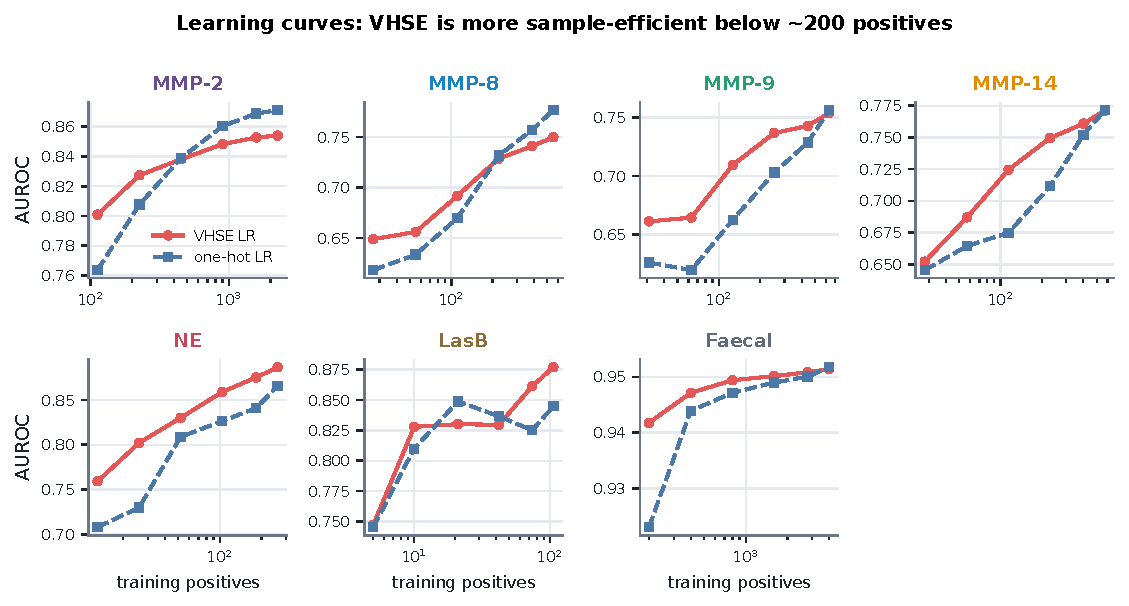
\includegraphics[width=\textwidth]{figures/F06_learning_curves.pdf}
\caption{Learning curves: AUROC as a function of the number of training positives for the VHSE and one-hot logistic regressions. The physicochemical encoding is more sample-efficient at small sizes.}
\label{fig:lc}
\end{figure}

\subsection{Training against other proteases}
\label{sec:res-neg}
The training negatives determine what the model learns to reject. We compare three designs on a \emph{common} held-out test set, trained inside identical folds: (i) composition-shuffled positives plus background (the design used in earlier work), (ii) background only, and (iii) our panel design. Each is scored on held-out target positives against (a) background windows and (b) held-out positives of the other proteases (Table~\ref{tab:neg}, Figure~\ref{fig:neg}). The panel design costs $0.01$--$0.02$ AUROC against background but gains against competitors on every protease, most where it matters: for LasB from $0.80$ (background only) and $0.68$ (shuffled) to $0.86$, for MMP-14 from $0.65$ to $0.73$, and for MMP-2 from $0.76$ to $0.79$.

\begin{table}[!htbp]
\centering\small\begin{tabular}{@{}lcccccc@{}}\toprule
 & \multicolumn{2}{c}{Shuffled + background} & \multicolumn{2}{c}{Background only} & \multicolumn{2}{c}{Panel (ours)} \\
\cmidrule(lr){2-3}\cmidrule(lr){4-5}\cmidrule(lr){6-7}
Protease & vs bkg & vs comp. & vs bkg & vs comp. & vs bkg & vs comp. \\\midrule
MMP-2 & 0.881 & 0.756 & 0.885 & 0.762 & 0.882 & 0.787 \\
MMP-8 & 0.834 & 0.654 & 0.828 & 0.651 & 0.810 & 0.683 \\
MMP-9 & 0.819 & 0.660 & 0.832 & 0.667 & 0.816 & 0.683 \\
MMP-14 & 0.831 & 0.660 & 0.833 & 0.649 & 0.811 & 0.727 \\
Neutrophil elastase & 0.850 & 0.910 & 0.852 & 0.900 & 0.848 & 0.926 \\
LasB & 0.801 & 0.676 & 0.889 & 0.798 & 0.891 & 0.863 \\
Faecal serine proteases & 0.954 & 0.939 & 0.954 & 0.938 & 0.953 & 0.944 \\
\bottomrule\end{tabular}

\caption{Held-out AUROC by negative-set design against random background (bkg) and against other proteases' substrates (comp.).}
\label{tab:neg}
\end{table}

\begin{figure}[!htbp]
\centering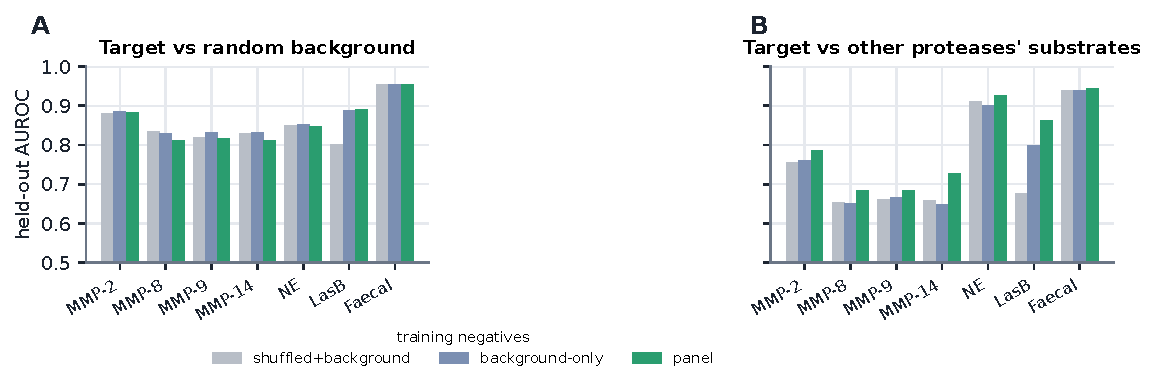
\includegraphics[width=\textwidth]{figures/F07_negative_design.pdf}
\caption{Effect of the training negatives on detection (a) and cross-protease discrimination (b).}
\label{fig:neg}
\end{figure}

\subsection{Regularisation, leakage and controls}
Choosing $C$ by inner cross-validation raises or matches the $C=1$ default (Table~\ref{tab:controls}, Figure~\ref{fig:tune}), selecting $C=0.01$--$0.1$ for every protease except the faecal group (strong regularisation for a $64$-feature model on hundreds of examples). Random and cluster-aware folds differ by at most \maxLeakGap{} AUROC, so near-duplicate leakage is not a material source of optimism in these data, even though the folds guard against it. Label-shuffled models score \shuffleMin--\shuffleMax{}.

\begin{table}[!htbp]
\centering\small\begin{tabular}{@{}lcccccc@{}}\toprule
 & \multicolumn{2}{c}{Regularisation} & \multicolumn{2}{c}{Fold construction} & Label & VHSE span \\
\cmidrule(lr){2-3}\cmidrule(lr){4-5}
Protease & $C=1$ & nested & random & clustered & shuffle & coverage \\\midrule
MMP-2 & 0.854 & 0.854 & 0.855 & 0.854 & 0.505 & 79\% \\
MMP-8 & 0.750 & 0.755 & 0.752 & 0.752 & 0.493 & 64\% \\
MMP-9 & 0.754 & 0.760 & 0.755 & 0.756 & 0.493 & 64\% \\
MMP-14 & 0.771 & 0.772 & 0.771 & 0.773 & 0.509 & 79\% \\
Neutrophil elastase & 0.887 & 0.895 & 0.897 & 0.895 & 0.495 & 65\% \\
LasB & 0.877 & 0.877 & 0.886 & 0.879 & 0.526 & 65\% \\
Faecal serine proteases & 0.951 & 0.951 & 0.951 & 0.951 & 0.494 & 77\% \\
\bottomrule\end{tabular}

\caption{Controls. Regularisation: AUROC with $C=1$ versus $C$ chosen in the inner loop. Fold construction: random versus cluster-aware folds (fixed $C=0.1$). Label shuffle: mean over five permutations. VHSE span: variance-weighted share of the learned PSSM log-odds that lies within the VHSE subspace.}
\label{tab:controls}
\end{table}

\begin{figure}[!htbp]
\centering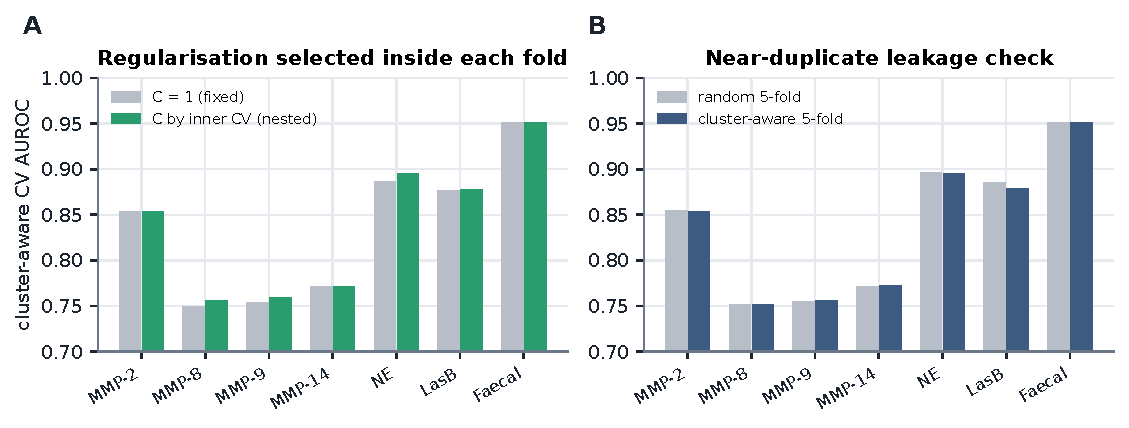
\includegraphics[width=\textwidth]{figures/F08_tuning_and_leakage.pdf}
\caption{\textbf{(a)} Nested regularisation selection versus fixed $C=1$. \textbf{(b)} Random versus cluster-aware folds.}
\label{fig:tune}
\end{figure}

\subsection{Calibration and scale}
\label{sec:res-calib}
Reliability curves of the logistic-regression score lie below the diagonal (Figure~\ref{fig:calib}a): with balanced class weights the score is a posterior under a $50{:}50$ prior, whereas the training mixture has a positive prior of $0.25$ and real sequences far lower. Expected calibration error is $0.06$--$0.20$ (Table~\ref{tab:secondary}). Base rates also differ by model: the mean score on random windows ranges from $0.11$ (faecal) to $0.35$ (MMP-14) (Figure~\ref{fig:calib}b), which is precisely what makes raw probability ratios unsuitable as selectivity measures and motivates the percentile scale.

\begin{figure}[!htbp]
\centering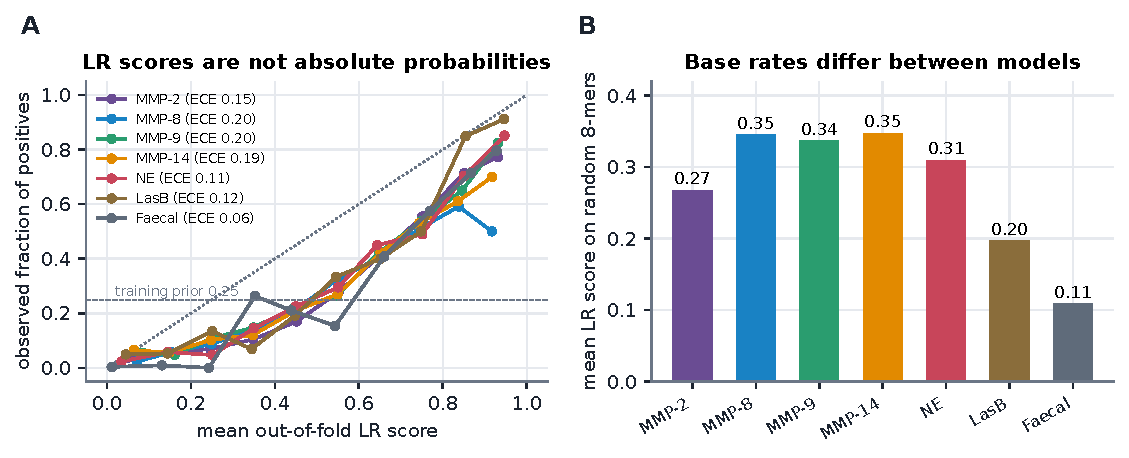
\includegraphics[width=\textwidth]{figures/F10_calibration.pdf}
\caption{\textbf{(a)} Reliability curves of the out-of-fold logistic-regression score. \textbf{(b)} Mean logistic-regression score on random background windows for each final model.}
\label{fig:calib}
\end{figure}

\subsection{Selectivity between proteases}
\label{sec:res-sel}
Table~\ref{tab:selmat} and Figure~\ref{fig:selmat} report, for each target model, the held-out AUROC for separating the target's substrates from a competitor's substrates (the competitor's windows were in training as negatives, but each is scored out-of-fold). The pattern follows the biology of Section~\ref{sec:bio}. The NE and faecal models separate their own substrates from every competitor's at $0.90$--$0.98$. The MMP models separate theirs from NE's at $0.89$--$0.93$, but from LasB's and the faecal group's at only $0.63$--$0.89$. And \emph{within} the MMP family discrimination is modest ($0.53$--$0.72$), lowest for MMP-14 versus MMP-2 ($0.53$) and MMP-8 versus MMP-2 ($0.57$).

\begin{table}[!htbp]
\centering\small\begin{tabular}{@{}lccccccc@{}}\toprule
Target model & MMP-2 & MMP-8 & MMP-9 & MMP-14 & NE & LasB & Faecal \\\midrule
MMP-2 & -- & 0.72 & 0.68 & 0.69 & 0.93 & 0.79 & 0.89 \\
MMP-8 & 0.57 & -- & 0.58 & 0.64 & 0.91 & 0.82 & 0.63 \\
MMP-9 & 0.59 & 0.65 & -- & 0.70 & 0.90 & 0.63 & 0.63 \\
MMP-14 & 0.53 & 0.62 & 0.70 & -- & 0.89 & 0.80 & 0.84 \\
Neutrophil elastase & 0.93 & 0.93 & 0.93 & 0.94 & -- & 0.92 & 0.96 \\
LasB & 0.84 & 0.90 & 0.81 & 0.84 & 0.87 & -- & 0.91 \\
Faecal & 0.96 & 0.90 & 0.91 & 0.96 & 0.98 & 0.97 & -- \\
\bottomrule\end{tabular}

\caption{Held-out AUROC for separating the row protease's substrates from the column protease's substrates.}
\label{tab:selmat}
\end{table}

\begin{figure}[!htbp]
\centering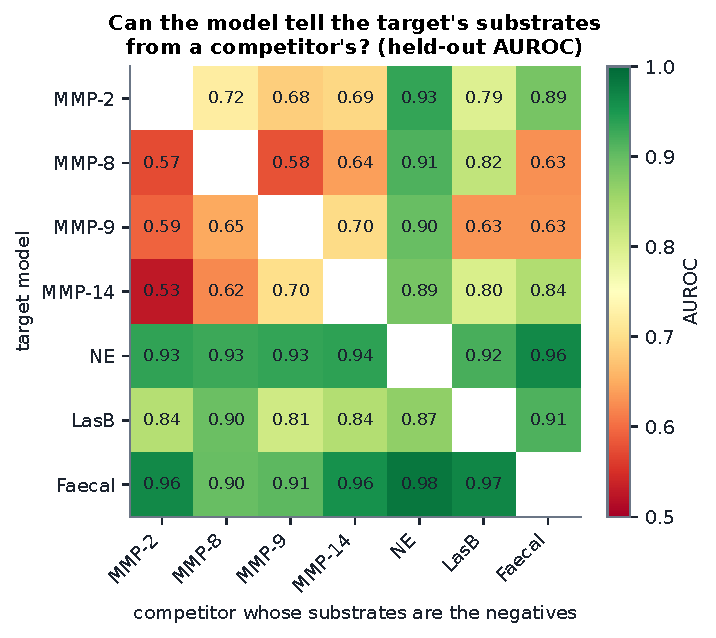
\includegraphics[width=0.62\textwidth]{figures/F11_selectivity_matrix.pdf}
\caption{Cross-protease discrimination matrix (same data as Table~\ref{tab:selmat}).}
\label{fig:selmat}
\end{figure}

\subsubsection{How to read a low competitor AUROC}
\label{sec:contam}
A low value does not by itself indicate a poor model. By Eq.~\eqref{eq:contam-main}, if a fraction $\pi$ of a competitor's substrates are also cleaved by the target, the measured AUROC is at most $(1-\pi)\cdot1+\tfrac12\pi=1-\pi/2$ even for a perfect model. Exact-window overlap between protease positive sets is small (Section~\ref{sec:data}), but the MMPs share their dominant preferences (Section~\ref{sec:bio}), so many unlabelled or ``competitor'' windows are plausibly cleaved by the target as well; the ceiling for MMP-versus-MMP AUROC is therefore below $1$ by an amount we cannot measure from sequence data alone. In other words, part of the within-MMP figure reflects genuine biological promiscuity in the labels. Either way, the practical conclusion is the same: from a P4--P4$'$ window alone, the MMPs cannot be reliably told apart, and a sensor design should not depend on it.

\begin{figure}[!htbp]
\centering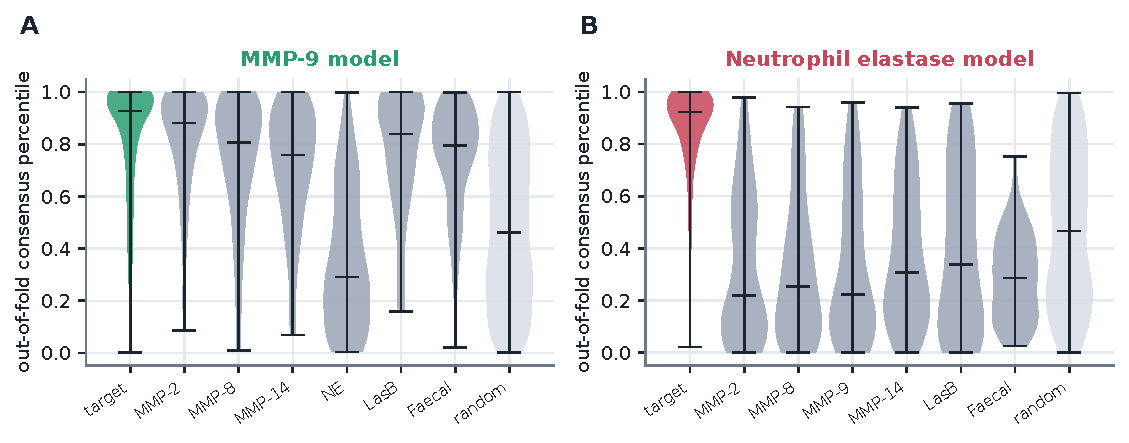
\includegraphics[width=\textwidth]{figures/F16_score_distributions.pdf}
\caption{Out-of-fold consensus percentiles of held-out positives (``target'') and of each competitor's substrates and random windows, for the MMP-9 model (a) and the NE model (b). The MMP-9 model places MMP-2 and MMP-8 substrates almost as high as its own; the NE model separates them sharply.}
\label{fig:dist}
\end{figure}

\subsection{What the models learned}
\label{sec:interp}
Coefficient stability by cluster bootstrap (Figure~\ref{fig:coef}) shows which learned effects are reliable: between $17$ (MMP-14) and $35$ (MMP-2) of the $64$ standardised coefficients per model have intervals excluding zero, so most individual coefficients are not reliably nonzero and the position-level pattern is more trustworthy than any single descriptor weight. Figure~\ref{fig:pos} shows that the total contribution is concentrated at $\pos{3}$ and $\prm{1}$ for the MMPs, at $\pos{1}$ for NE and the faecal group, and is spread across positions for LasB; the electronic family, which accounts for four of the eight descriptors, carries the largest share for every protease.

\begin{figure}[!htbp]
\centering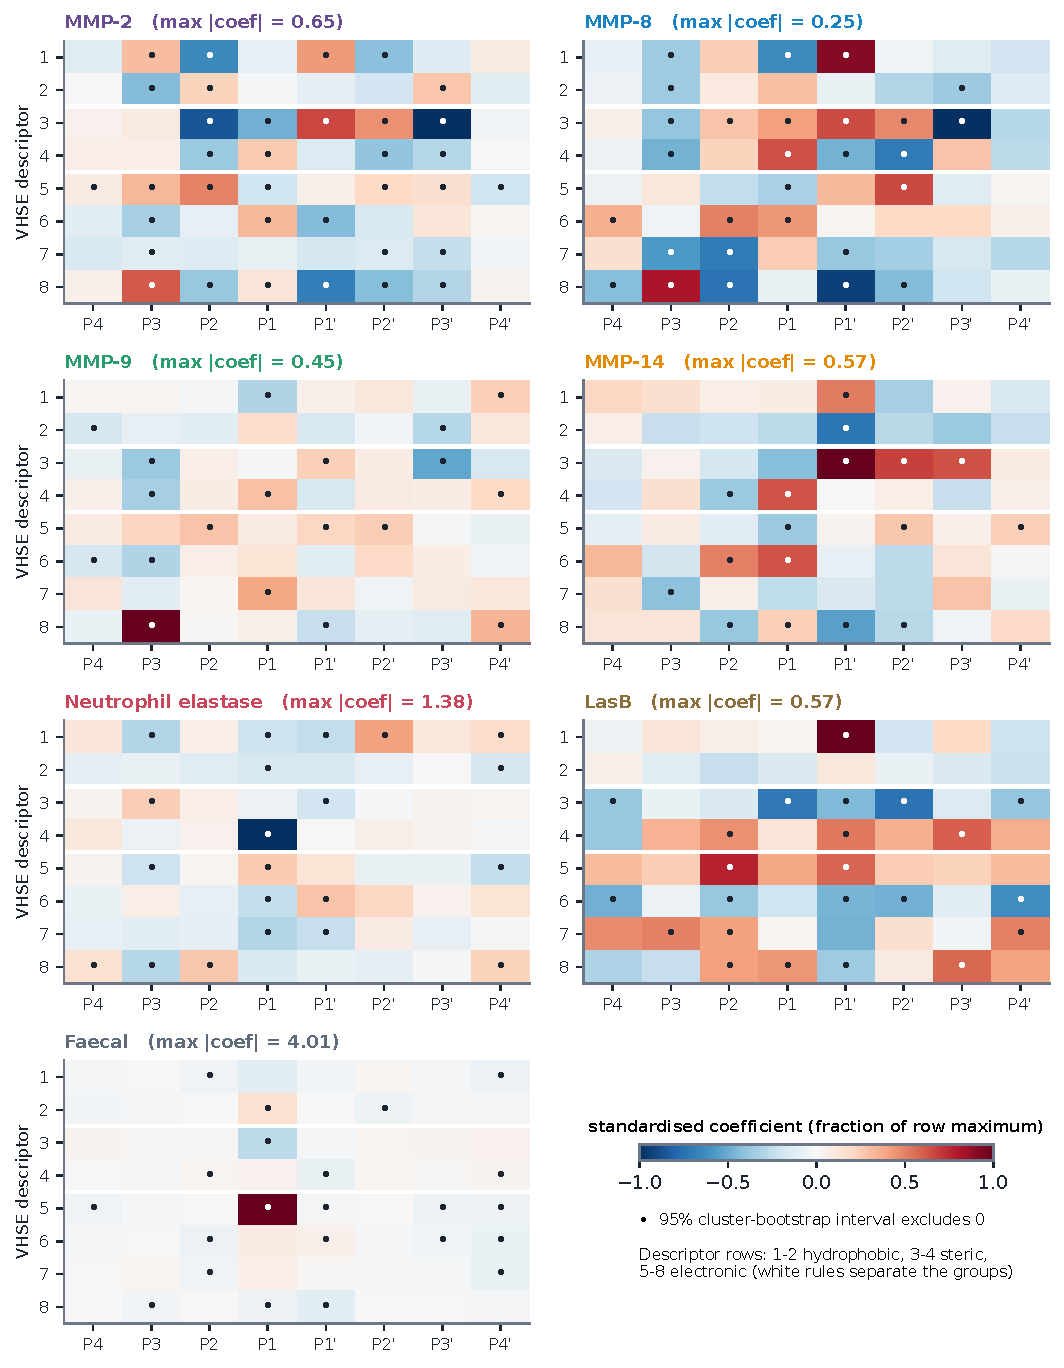
\includegraphics[width=0.97\textwidth]{figures/F12_coefficients.pdf}
\caption{Standardised logistic-regression coefficients by position and VHSE descriptor. Dots mark coefficients whose $95\%$ cluster-bootstrap interval excludes zero. Colours are scaled to each protease's largest coefficient.}
\label{fig:coef}
\end{figure}

\begin{figure}[!htbp]
\centering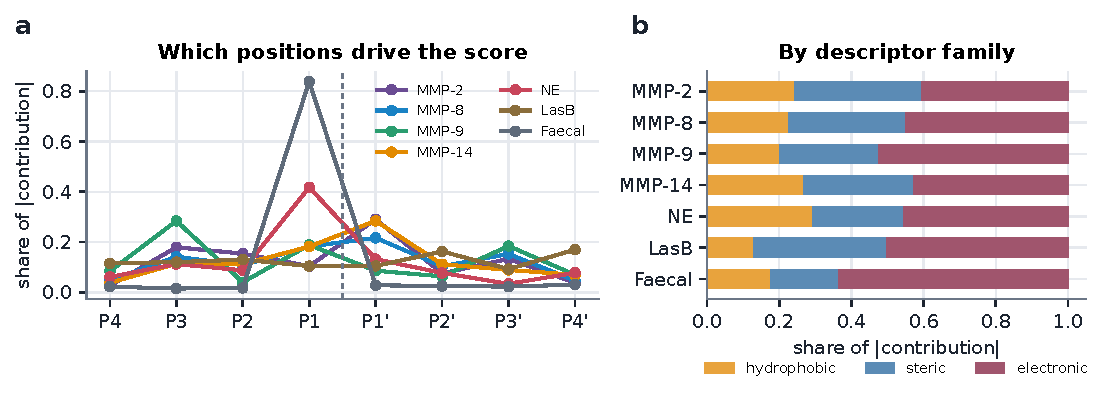
\includegraphics[width=\textwidth]{figures/F13_position_importance.pdf}
\caption{\textbf{(a)} Share of mean absolute logit contribution by position, computed on training positives. \textbf{(b)} Share by descriptor family.}
\label{fig:pos}
\end{figure}
